\begin{figure*}[tp]
\centering
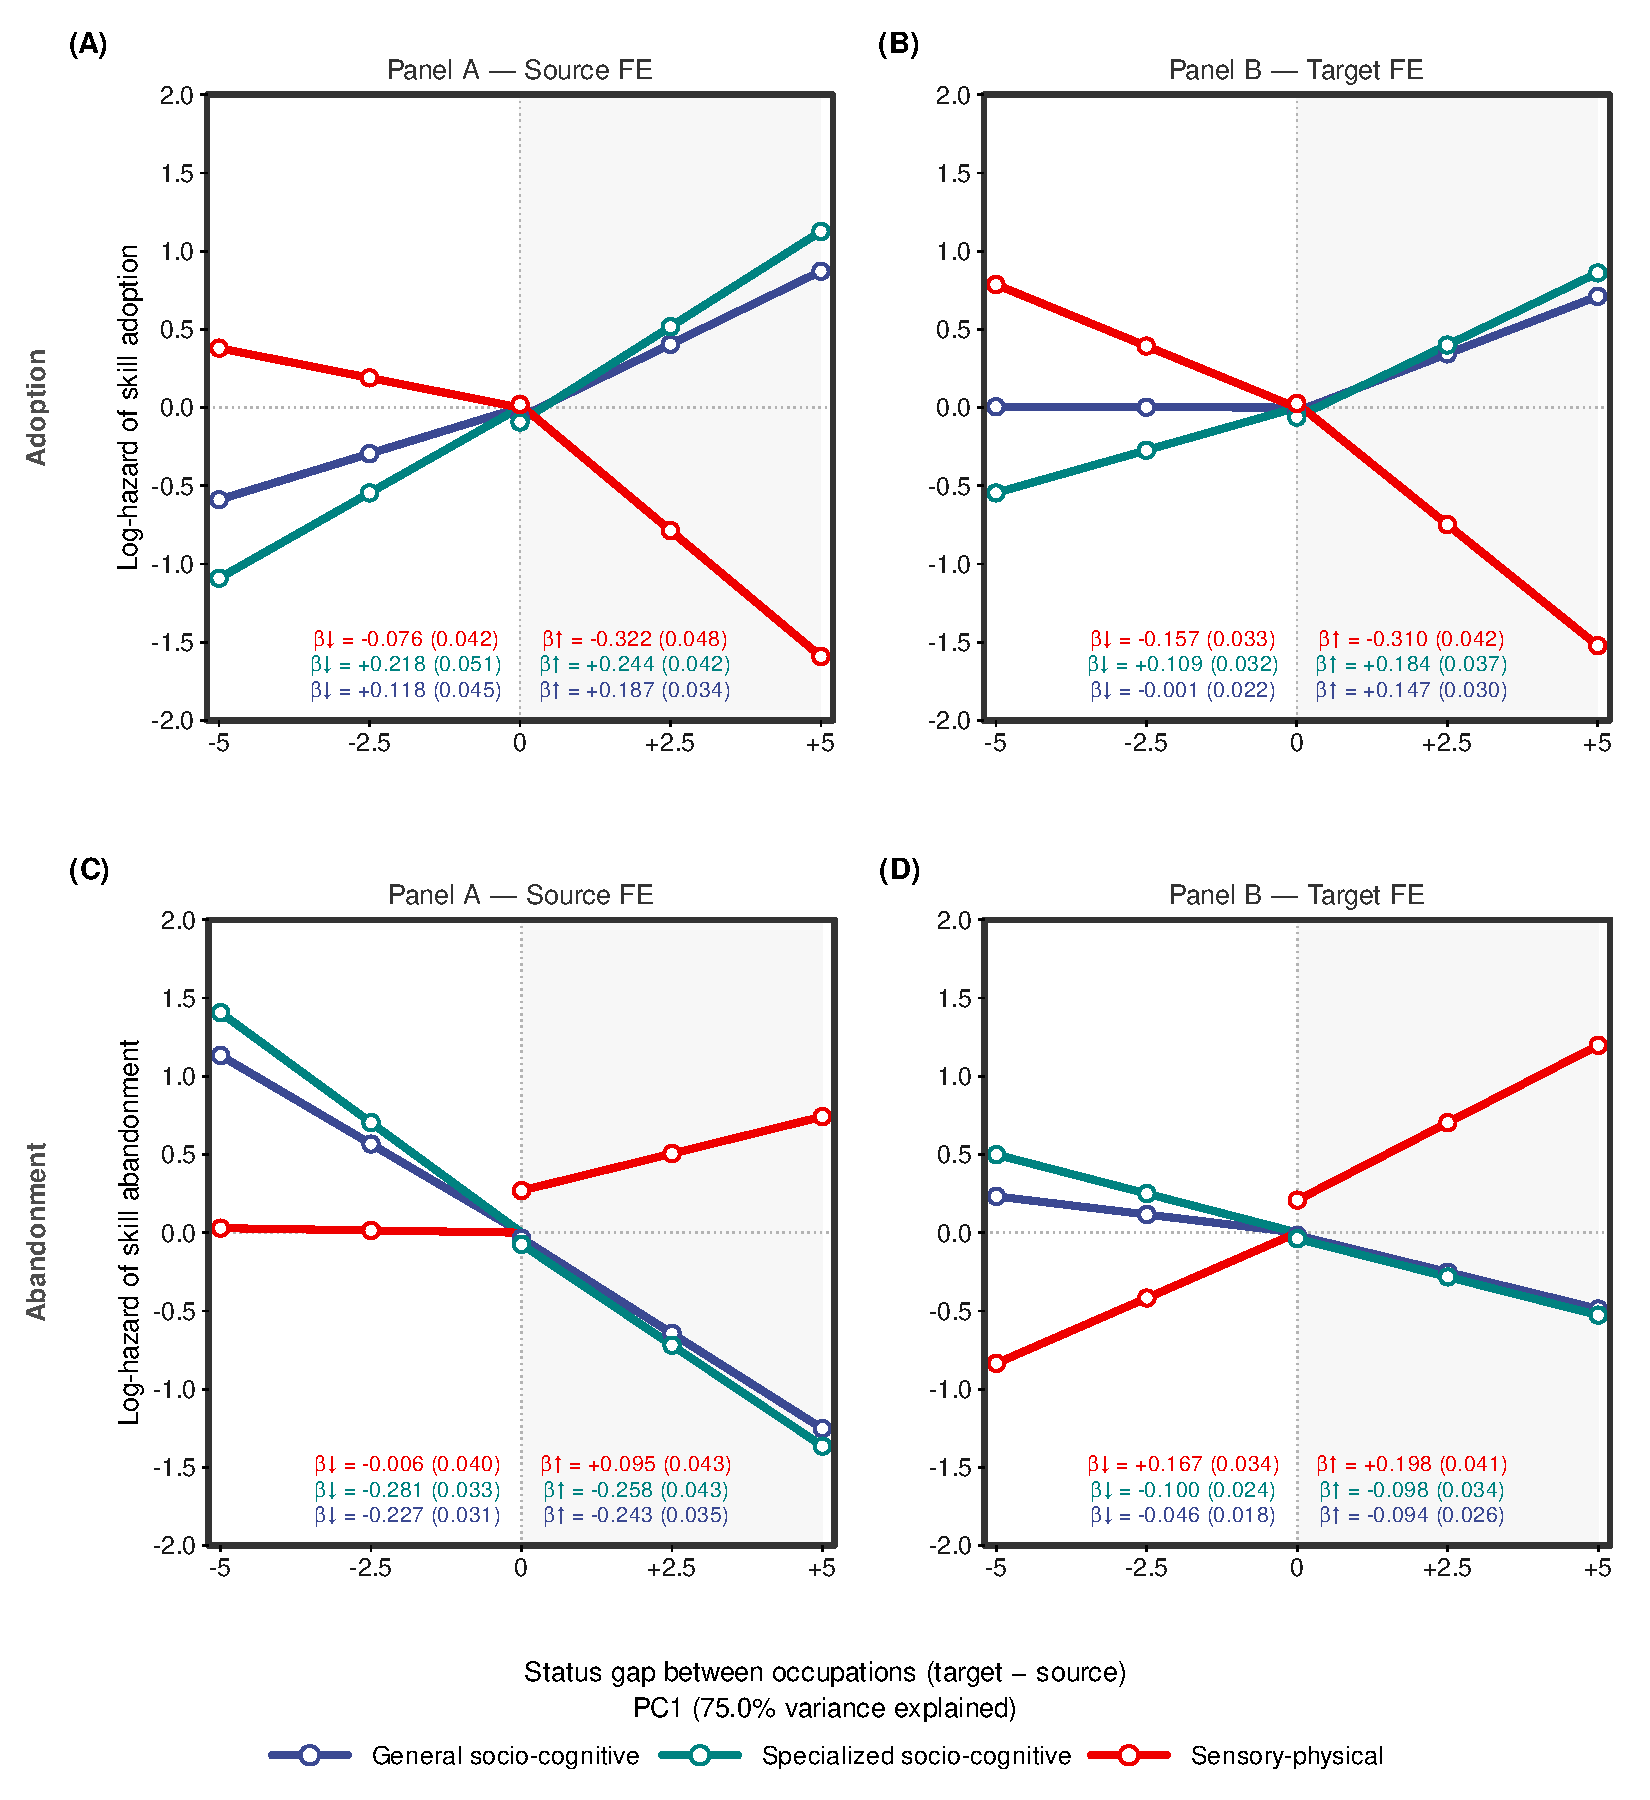
\includegraphics[width=0.90\linewidth]{figures/fig2_regression.pdf}
\caption{%
\textbf{Fitted log-hazard of skill adoption and abandonment as a function of signed status gap, under two complementary fixed-effect strategies.}
Colors distinguish three skill types throughout: \textcolor[HTML]{3B4992}{\textbf{general socio-cognitive}}, \textcolor[HTML]{008280}{\textbf{specialized socio-cognitive}}, and \textcolor[HTML]{EE0000}{\textbf{sensory-physical}}. The horizontal axis across all panels represents the composite PC1 status gap (target minus source). The unshaded region (left of $G_{ij}=0$) corresponds to downward gaps (target ranks below source), while the gray-shaded region (right) corresponds to upward gaps (target ranks above source). The vertical axis is the log-hazard from the complementary log-log gravity model (Eq.~\ref{eq:gravity_main}).
\textbf{(A, B)}~Skill adoption under source and skill fixed effects (A), identifying the gap effect from variation across targets, and under target and skill fixed effects (B), identifying it from variation across sources.
\textbf{(C, D)}~Skill abandonment under the same two strategies: source and skill fixed effects (C) and target and skill fixed effects (D).
\textbf{Visual encodings:} Solid lines represent the fitted piecewise linear predictor evaluated along the status gap. Open circles mark predicted values at 2.5-unit reference intervals ($-5$, $-2.5$, $0$, $+2.5$, $+5$). In-plot text annotations report the estimated slopes for downward ($\hat{\beta}^{\downarrow}$) and upward ($\hat{\beta}^{\uparrow}$) gaps by skill class, with standard errors in parentheses (clustered three-way by source occupation, target occupation, and skill). The rug plot beneath the horizontal axis displays the distribution of dyad-level status gaps for a random subsample of 60{,}000 dyads per flow. Adoption: $n\approx21.5$\,M directed dyads; Abandonment: $n\approx18.6$\,M. O*NET, 2015--2024.
}
\label{fig:model_projection_combined}
\end{figure*}
